\documentclass[tikz]{standalone}
\usetikzlibrary{arrows.meta,positioning}

\begin{document}
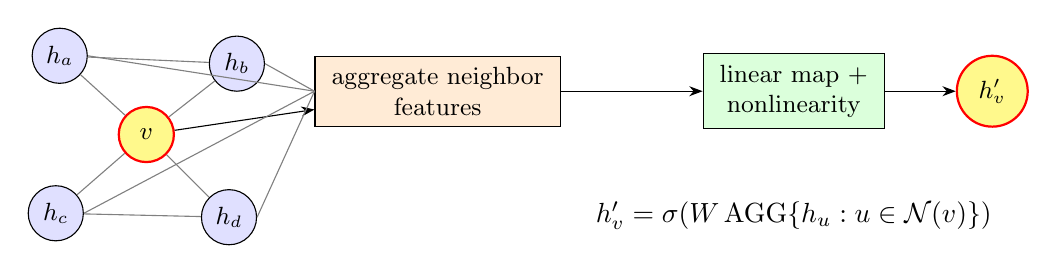
\begin{tikzpicture}[
  >=Stealth,
  vtx/.style={circle,draw,minimum size=7mm,inner sep=0,font=\small},
  block/.style={draw,align=center,inner xsep=6pt,inner ysep=4pt,font=\small},
]
  \node[vtx,fill=yellow!45,draw=red,thick] (v) at (0,0) {$v$};
  \foreach \n/\x/\y in {a/-1.1/1,b/1.15/.9,c/-1.15/-1,d/1.05/-1.05}
    \node[vtx,fill=blue!12] (\n) at (\x,\y) {$h_\n$};
  \foreach \a/\b in {v/a,v/b,v/c,v/d,a/b,c/d} \draw[gray] (\a) -- (\b);
  \node[block,fill=orange!16] (agg) at (3.7,.55) {aggregate neighbor\\features};
  \node[block,fill=green!14,right=18mm of agg] (map) {linear map +\\nonlinearity};
  \node[vtx,fill=yellow!45,draw=red,thick,minimum size=9mm,right=9mm of map] (out) {$h'_v$};
  \foreach \a/\b in {v/agg,agg/map,map/out} \draw[->] (\a) -- (\b);
  \foreach \n in {a,b,c,d} \draw[gray] (\n.east) -- (agg.west);
  \node[below=8mm of map] {$h'_v=\sigma\!\left(W\,\mathrm{AGG}\{h_u:u\in\mathcal N(v)\}\right)$};
\end{tikzpicture}
\end{document}
